\documentclass[11pt]{article}

\usepackage[margin=1in]{geometry}
\usepackage{amsmath,amssymb}
\usepackage{graphicx}
\usepackage{booktabs}
\usepackage{xcolor}
\usepackage{hyperref}
\hypersetup{colorlinks=true, linkcolor=blue, citecolor=blue, urlcolor=blue}
\usepackage{caption}
\usepackage{authblk}

\newcommand{\SBA}{S(B|A)}
\newcommand{\Strue}{S_{\rm true}}
\newcommand{\Itrue}{I_{\rm true}}

\title{Quantum vs.\ Classical Correlations in Dijet Hadron Multiplicities:\\
A Finite-Statistics Methodology Note}

\author[1,2]{Zhoudunming (Kong) Tu}
\affil[1]{Brookhaven National Laboratory}
\affil[2]{Stony Brook University}

\date{\today}

\begin{document}
\maketitle

\begin{abstract}
\noindent
We work through the full methodological chain for measuring mutual
information (MI) between back-to-back jets from hadron multiplicity
distributions, and for establishing whether an observed correlation could
be a genuine quantum signature or is fully explained by classical physics
plus finite-sample statistical bias. We show that the naive plug-in
entropy/MI estimator is systematically biased upward at finite event
count~$N$, in exactly the direction that could be mistaken for a quantum
excess if left uncorrected. Using a controlled Monte Carlo toy model with
a known ground truth, we validate two standard corrections (Miller--Madow
and shuffle-subtraction) and a more rigorous Bayesian estimator (NSB,
Nemenman--Shafee--Bialek), and use the best-behaved of these to derive a
concrete, quantitative detection-sensitivity curve: how large a genuine
quantum-correlation excess must be, at a given event count, to be
statistically distinguishable from finite-sample noise.
\end{abstract}

\tableofcontents

% =============================================================================
\section{Physics motivation}
% =============================================================================

Take a back-to-back dijet event (e.g.\ from $e^+e^-$, DIS, or $pp$
collisions at RHIC/STAR). Treat jet $A$ and jet $B$ as the two subsystems
of a bipartite system whose ``state'' is accessed only through observed
hadron multiplicities, via \textbf{local parton--hadron duality (LPHD)}:
the hadron multiplicity distribution stands in for the underlying parton
Fock-state distribution.

\textbf{The Schmidt-decomposition ansatz} (Kharzeev--Levin;
Peschanski--Seki): if each Fock/parton-number sector $n$ carries
probability $P(n)$, and the reduced density matrix of a jet is diagonal in
$n$, then the entanglement entropy of that jet reduces to the
\textbf{Shannon entropy of its hadron multiplicity distribution},
\begin{equation}
S_A = -\sum_n P_A(n)\ln P_A(n),
\end{equation}
and likewise for $S_B$. This turns a genuinely quantum quantity
(entanglement entropy) into something directly measurable from ordinary
multiplicity counting -- the whole program rests on this ansatz.

\textbf{The physics question:} by additionally measuring the \emph{joint}
multiplicity distribution $P_{AB}(n_A,n_B)$ across both jets in the same
event, we can construct the mutual information $I(A{:}B)$ between the two
jets (defined in Sec.~\ref{sec:observable}). A large enough MI, in the
right combination with the individual entropies, would signal
correlations between the jets that cannot be explained by any classical
joint probability distribution -- i.e.\ a genuine quantum (entanglement)
signature surviving from the partonic state through hadronization, rather
than an ordinary classical correlation (e.g.\ shared color flow, momentum
conservation, or other QCD-driven but fundamentally classical
correlations).

\textbf{Why this is subtle in practice:} any such claim is only as good as
(a) correctly separating genuine quantum correlation from unavoidable
classical correlation, and (b) correctly accounting for the finite size of
real data samples, since MI estimated from a finite event sample is
\textbf{always statistically biased}, and -- as we show below -- biased in
exactly the direction that could be mistaken for a quantum excess if not
handled carefully. This note works through both issues end to end.

% =============================================================================
\section{The observable: MI, conditional entropy, and the quantum witness}
\label{sec:observable}
% =============================================================================

From the per-jet and joint hadron-multiplicity distributions we can build
three entropies and two derived quantities:
\begin{equation}
S_A,\quad S_B,\quad S_{AB}
\qquad\Longrightarrow\qquad
I(A{:}B) = S_A+S_B-S_{AB},
\qquad
\SBA = S_{AB}-S_A .
\end{equation}

\paragraph{Mutual information alone cannot distinguish quantum from
classical.} $I(A{:}B)>0$ just means the jets are correlated \emph{somehow}
-- a purely classical joint distribution (shared color flow,
energy--momentum conservation, any ordinary QCD dynamics) also gives
nonzero MI. A sharper diagnostic is needed.

\paragraph{The sharper test: conditional entropy negativity.} For
\emph{any} classical discrete probability distribution, Shannon
conditional entropy obeys
\begin{equation}
\SBA = S_{AB}-S_A \;\geq\; 0 \qquad \text{(always, classically).}
\end{equation}
This is the classical subadditivity of Shannon entropy -- not an
assumption about any particular physical model. Only the \emph{quantum}
(von Neumann) conditional entropy can go negative, and only for entangled
states. So \textbf{$\SBA<0$ is a hard classical impossibility}, and
observing it (at sufficient statistical significance) would be direct
evidence that the jets cannot be described by a classical joint
probability distribution -- i.e.\ a genuine quantum signature.
Equivalently, in terms of MI alone,
\begin{equation}
I(A{:}B) \;>\; \min(S_A,S_B)
\qquad\Longleftrightarrow\qquad
\SBA<0 \ \text{ or }\ S(A|B)<0,
\end{equation}
so MI exceeding the smaller of the two marginal entropies is the same
statement in a different form. Both directions ($\SBA$ and $S(A|B)$) are
worth checking independently, since conditional entropy is not symmetric.

\paragraph{What this test cannot do: genuine quantum discord.} True
(Ollivier--Zurek) quantum discord is defined by optimizing conditional
entropy over \emph{quantum measurement bases} -- non-commuting projective
measurements that don't reduce to simply reading off a classical value.
Hadron-multiplicity data $(N_A,N_B)$ is, by construction, a classical
joint distribution (a histogram). For any classical joint distribution,
the optimal ``measurement'' on $B$ is trivially just observing $N_B$
exactly, which makes the classical-correlation piece $J(A{:}B)$ equal to
the \emph{full} $I(A{:}B)$ exactly -- so discord $D=I-J\equiv 0$
identically, for any classical distribution, with no exception. Extracting
a genuinely nonzero discord requires actual quantum-state tomography
(e.g.\ the $\Lambda\bar\Lambda$ spin-density-matrix channel), not
multiplicity counting. \textbf{The conditional-entropy-negativity test
above is therefore the correct and complete witness available from this
kind of data} -- the rest of this note is about measuring it reliably.

% =============================================================================
\section{The statistical problem: finite-sample bias}
\label{sec:bias}
% =============================================================================

Every quantity above is estimated from a finite event sample, and the
naive (``plug-in'') entropy estimator has a \textbf{systematic, structural
bias} that turns out to point in exactly the dangerous direction for this
measurement.

\paragraph{Where the bias comes from.} The naive estimator replaces true
probabilities $p_i$ with empirical frequencies $\hat p_i=n_i/N$,
\begin{equation}
\hat S = -\sum_i \hat p_i \ln \hat p_i .
\end{equation}
Because $x\ln x$ is convex (equivalently $-x\ln x$ is concave), Jensen's
inequality guarantees
\begin{equation}
\langle \hat S \rangle \;<\; \Strue \qquad \text{for any finite } N,
\end{equation}
i.e.\ the plug-in estimator always underestimates entropy. This isn't a
numerical artifact; with only $N$ draws one can never fully resolve a
distribution's tails, and that missing resolution always looks like
\emph{less} apparent randomness than there truly is.

\paragraph{Leading-order size of the effect} (Miller 1955; Madow), for a
distribution over $K$ possible outcomes:
\begin{equation}
\langle \hat S \rangle \approx \Strue - \frac{K-1}{2N}.
\end{equation}
Fewer events ($N$ small) or finer binning ($K$ large) both make the
downward bias worse.

\paragraph{Why this flips sign and biases $I(A{:}B)$ upward.} Combining
the individual biases of $\hat S_A,\hat S_B,\hat S_{AB}$ with correct
signs,
\begin{equation}
\langle\hat I\rangle \;\approx\; \Itrue +
\frac{(K_{AB}-1)-(K_A-1)-(K_B-1)}{2N}
= \Itrue + \frac{K_{AB}-K_A-K_B+1}{2N}.
\label{eq:mi-bias}
\end{equation}
The joint distribution lives in a much larger space than either marginal
alone, so $\hat S_{AB}$ suffers a \emph{much larger} downward bias than
$\hat S_A+\hat S_B$ does -- and since $S_{AB}$ enters with a
\textbf{minus} sign, its extra negative bias flips into a \textbf{positive}
bias on $\hat I$. In the extreme case $N \ll K_A K_B$ (badly undersampled
joint histogram), this produces large \emph{phantom} apparent mutual
information even for truly independent variables -- sampling noise alone
can masquerade as a real correlation, and by the same mechanism can
masquerade as evidence for the ``quantum'' side of the $\SBA<0$ test above
if not corrected.

A commonly-quoted shortcut version of Eq.~\eqref{eq:mi-bias} is
$(K_A-1)(K_B-1)/(2N)$; this is not a different formula, it is
Eq.~\eqref{eq:mi-bias} evaluated under the extra assumption
$K_{AB}=K_AK_B$, i.e.\ a fully and uniformly occupied joint space. That
assumption only holds for independent variables; for correlated data the
observed $K_{AB}$ is much smaller than $K_AK_B$ (the joint distribution
concentrates on a narrow ridge rather than filling the full grid), so this
shortcut badly \emph{overestimates} the bias -- a pitfall we hit directly
in Sec.~\ref{sec:corrections}.

\paragraph{Practical consequence.} Comparing the same underlying physics
across data samples of different size -- different STAR running periods,
different luminosity, different jet-cone or multiplicity binning choices
-- will report systematically different central MI (and $\SBA$) values
purely from this effect, with zero change in the actual QCD physics.
Secs.~\ref{sec:toymc}--\ref{sec:nsb} demonstrate this concretely with a
toy model and work through three ways to correct for it;
Sec.~\ref{sec:sensitivity} turns the corrected, best-behaved estimator
into a quantitative statement about how large a genuine quantum signal
would need to be, at a given event count, to be distinguishable from this
bias.

% =============================================================================
\section{Toy Monte Carlo test bed}
\label{sec:toymc}
% =============================================================================

To demonstrate the bias concretely and validate corrections against a
known ground truth, we use a controlled toy model: two back-to-back jets,
$A$ and $B$, with a shared latent hard-process fluctuation $\Lambda$
(e.g.\ fluctuating parton virtuality / initial-state energy scale) drawn
from a Gamma distribution. Conditional on $\Lambda$, each jet's hadron
multiplicity is Poisson distributed,
\begin{equation}
\Lambda \sim \mathrm{Gamma}(k,\theta), \qquad
N_A\,|\,\Lambda \sim \mathrm{Poisson}(\Lambda), \qquad
N_B\,|\,\Lambda \sim \mathrm{Poisson}(c\,\Lambda).
\end{equation}
Marginalizing over $\Lambda$ gives each jet a \textbf{Negative Binomial}
multiplicity distribution (the standard KNO-like form used for hadron
multiplicities), and the shared $\Lambda$ induces a genuine -- but purely
\textbf{classical} -- correlation between $N_A$ and $N_B$, i.e.\
$\Itrue>0$ with $\SBA_{\rm true}$ solidly positive, exactly as required
classically. This is a convenient sandbox: we know the true joint
distribution (to arbitrary precision, from a huge reference sample), so we
can measure the \emph{bias} of any estimator directly, and later measure
how large a genuine quantum excess would need to be to be distinguishable
from this classical baseline's own statistical noise. Parameters used
throughout: $k=3.0$, $\theta=8.0$, $c=0.9$ (giving
$\mathrm{corr}(N_A,N_B)\approx 0.88$).

\subsection{Demonstration: two samples, same true distribution, different
size}

We generate a ``small'' event sample ($N=500$; e.g.\ a single limited run
/ low-luminosity STAR-like dataset), a ``large'' event sample
($N=200{,}000$; high-statistics dataset), and a very large reference
sample ($N=5\times10^6$) to pin down $\Itrue$ -- all drawn from the
\emph{exact same underlying physics}.

\begin{table}[h]
\centering
\caption{Naive $\hat I$ for three samples of the same true physics.}
\begin{tabular}{lrrrrr}
\toprule
Sample & $N$ & $K_A$ & $K_B$ & $K_{AB}$ & $\hat I_{\rm naive}$ (nats) \\
\midrule
small & 500 & 67 & 60 & 390 & 1.7424 \\
large & 200{,}000 & 129 & 113 & 3949 & 0.7463 \\
reference & 5{,}000{,}000 & 159 & 147 & 7022 & 0.7329 $\;(\approx \Itrue)$ \\
\bottomrule
\end{tabular}
\end{table}

We see $\hat I_{\rm small} > \hat I_{\rm large} \approx \hat I_{\rm ref}
\equiv \Itrue$ -- \textbf{the same physics, analyzed with fewer events,
reports a systematically larger MI}. This is the bias predicted in
Sec.~\ref{sec:bias}, not a change in physics.

The bias comes entirely from how well-populated the joint histogram is.
Figure~\ref{fig:marginals-joint} shows (top) the marginal
hadron-multiplicity distributions $P_A(n)$, overlaid for the three
samples -- these look reasonably similar even at $N=500$ because there are
only $O(10^2)$ bins to fill -- and (bottom) the 2D joint histograms
$P_{AB}(n_A,n_B)$ on the same color scale, where the difference is
dramatic: at $N=500$ the joint plane is almost empty, while at
$N=5\times10^6$ it is a smooth, fully-resolved correlated ridge. A sparse,
``salt-and-pepper'' joint histogram is exactly what drives $\hat S_{AB}$
artificially low, and hence $\hat I$ artificially high.

\begin{figure}[htb]
\centering
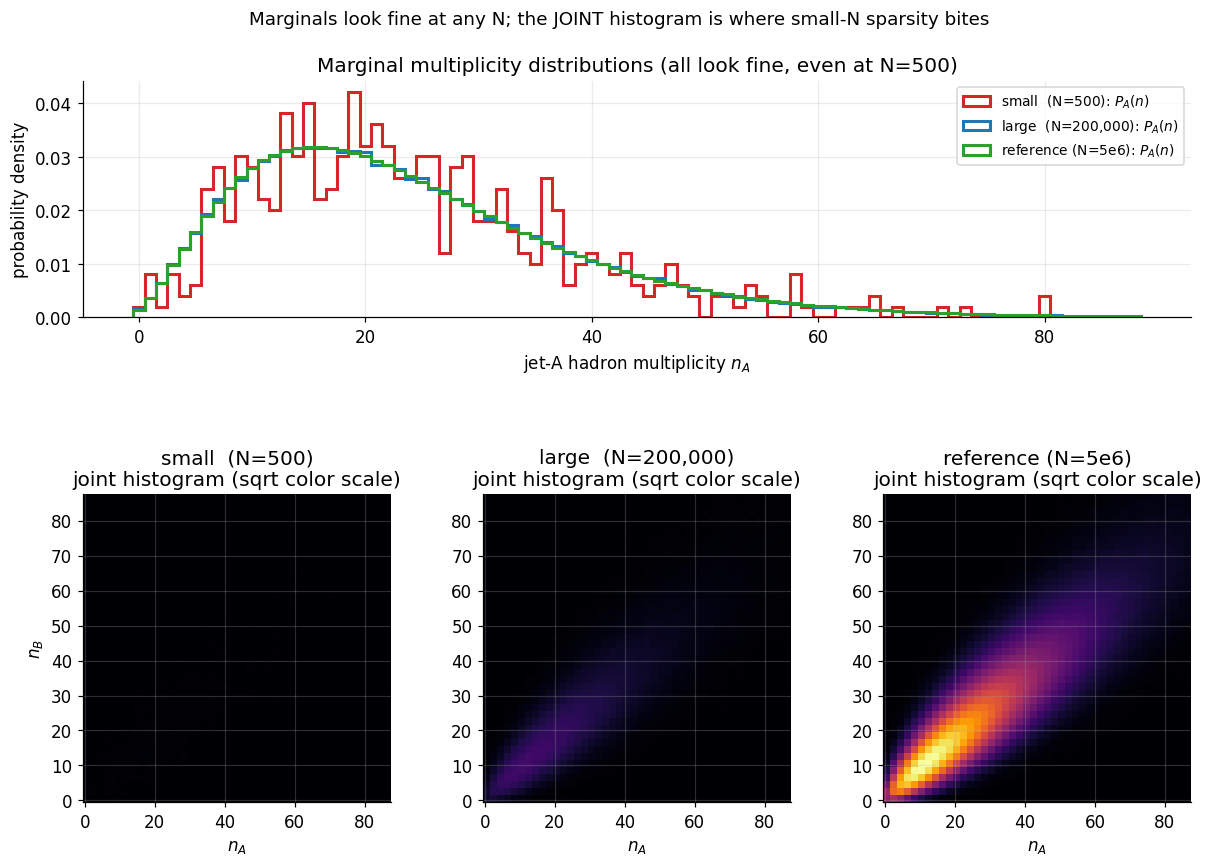
\includegraphics[width=\textwidth]{figs/fig01_marginals_joint.png}
\caption{Marginal multiplicity distributions (top) and 2D joint histograms
(bottom, square-root color scale) for the small, large, and reference
samples. Marginals look consistent at any $N$; the joint histogram is
where small-$N$ sparsity bites.}
\label{fig:marginals-joint}
\end{figure}

\subsection{Bias vs.\ sample size}

Repeating the naive estimate over a range of $N$ (with several repetitions
per $N$ to see the scatter) and plotting $\hat I_{\rm naive}$ against
$1/N$ (Fig.~\ref{fig:bias-vs-N}) shows the systematic downward drift
(bias shrinking) as $N$ grows, converging toward the flat reference line,
and the expected near-linear behavior in $1/N$: the intercept of that line
is a cheap, model-independent estimate of the bias-corrected/true MI. The
extrapolated intercept, $0.9427$ nats, lands reasonably close to the
reference value of $0.7329$ nats.

\begin{figure}[htb]
\centering
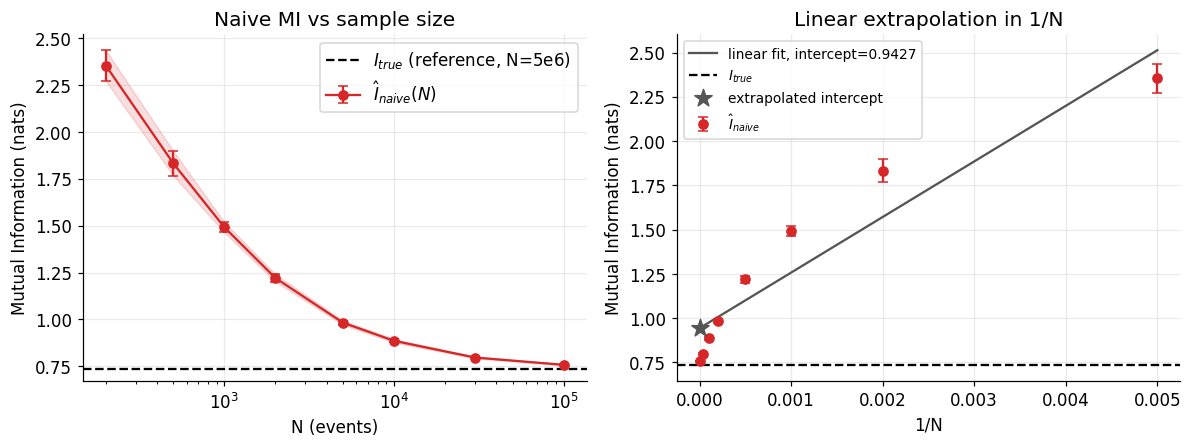
\includegraphics[width=\textwidth]{figs/fig02_bias_vs_N.png}
\caption{Left: naive $\hat I$ vs.\ sample size $N$, converging to the
reference value. Right: the same data plotted against $1/N$, with a linear
extrapolation to $1/N\to0$.}
\label{fig:bias-vs-N}
\end{figure}

% =============================================================================
\section{Corrections: Miller--Madow and shuffle-subtraction}
\label{sec:corrections}
% =============================================================================

\subsection{Miller--Madow correction}

The exact leading-order Miller--Madow correction applies the
$-(K-1)/(2N)$ term to \emph{each} of $S_A,S_B,S_{AB}$ separately and
combines them:
\begin{equation}
\hat I_{MM} = \hat I_{\rm naive} - \frac{(K_{AB}-1)-(K_A-1)-(K_B-1)}{2N}
= \hat I_{\rm naive} - \frac{K_{AB}-K_A-K_B+1}{2N}.
\end{equation}
Crucially, $K_{AB}$ here must be the \emph{actually observed} number of
occupied joint bins, not the product $K_AK_B$: for correlated variables
(our case, by construction) the joint distribution concentrates on a
narrow ridge and $K_{AB}\ll K_AK_B$, so using the product in place of the
observed value wildly overcorrects and can drive $\hat I_{MM}$ negative.

\subsection{Shuffle-subtraction (label-permutation null)}

Randomly permuting the $B$-jet labels relative to the $A$-jet labels
\emph{within the same sample} destroys any true correlation
($I_{\rm true,shuffled}=0$ by construction) while reproducing the same
finite-sample bias. Averaging over many shuffles gives a direct empirical
estimate of the bias to subtract:
\begin{equation}
\hat I_{\rm corrected} = \hat I_{\rm naive} -
\big\langle \hat I_{\rm shuffled}\big\rangle .
\end{equation}
This makes no asymptotic assumption and remains reliable even when
$N\lesssim K_AK_B$, where Miller--Madow starts to break down. It has its
own bias, however: shuffling spreads the joint distribution over
\emph{more} bins than the true correlated data occupies, so the shuffled
surrogate is \emph{more} undersampled than the real data at the same $N$.
Shuffle-subtraction therefore tends to systematically
\textbf{overestimate} the bias and \textbf{overcorrect}, pulling
$\hat I_{\rm corrected}$ below $\Itrue$ when the true correlation is
strong.

\begin{table}[h]
\centering
\caption{Naive, Miller--Madow, and shuffle-corrected $\hat I$ vs.\ $N$.}
\begin{tabular}{rrrrr}
\toprule
$N$ & $\hat I_{\rm naive}$ & $\hat I_{MM}$ & $\hat I_{\rm shuffle}$ & $\Itrue$ (ref.) \\
\midrule
200    & 2.2764 & 2.0889 & 0.0657 & 0.7329 \\
500    & 1.8694 & 1.6014 & 0.1436 & 0.7329 \\
1000   & 1.4271 & 1.1756 & 0.2422 & 0.7329 \\
2000   & 1.1873 & 0.9866 & 0.3809 & 0.7329 \\
5000   & 0.9766 & 0.8539 & 0.5592 & 0.7329 \\
20000  & 0.8259 & 0.7750 & 0.6792 & 0.7329 \\
\bottomrule
\end{tabular}
\end{table}

With the correct Miller--Madow formula (using the observed $K_{AB}$), both
corrections pull the small-$N$ estimates much closer to $\Itrue$ than the
naive value and stay well-behaved (no more diving negative). Neither lands
exactly on $\Itrue$ at very small $N$: Miller--Madow is only a
first-order truncation of the true bias expansion, and shuffle-subtraction
overcorrects when the true correlation is strong, as explained above. Both
effects shrink as $N$ grows.

The shuffle procedure gives more than a bias correction -- the spread of
$\hat I_{\rm shuffled}$ over many permutations \emph{is} the null
distribution for ``$\Itrue=0$'' at that $N$ and binning
(Fig.~\ref{fig:shuffle-null}). Plotting $\hat I_{\rm naive}$ against that
null distribution is a direct visual significance check: at $N=500$ the
null distribution itself is already centered well above zero (pure bias)
and the naive value sits close to or inside this null cloud, so on its own
it would not be significant evidence of correlation, even though the jets
are truly correlated by construction. By $N=20{,}000$ the null has
collapsed toward zero and the naive value clearly separates from it.

\begin{figure}[htb]
\centering
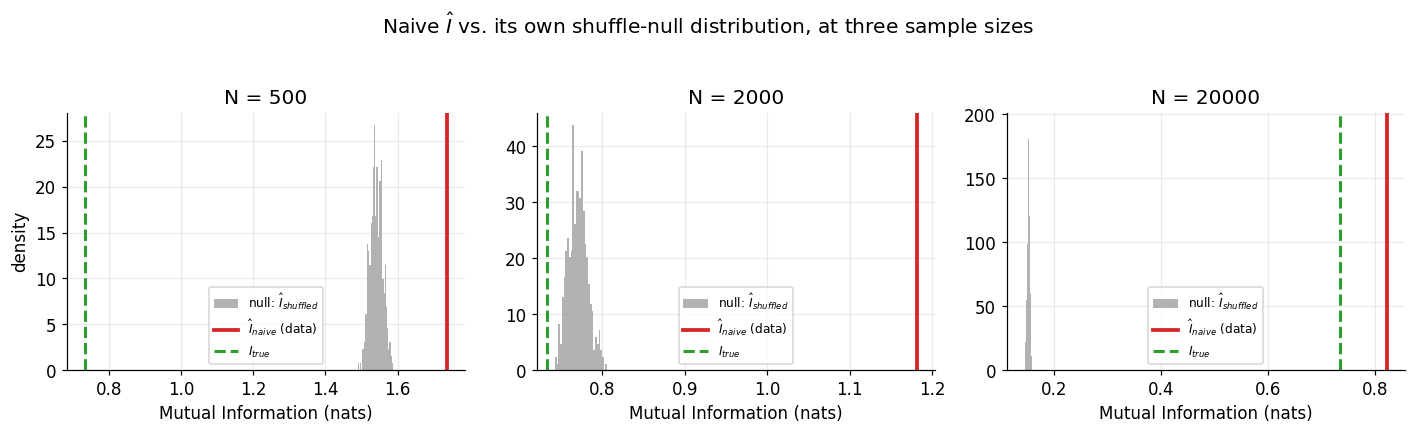
\includegraphics[width=\textwidth]{figs/fig03_shuffle_null.png}
\caption{Naive $\hat I$ (vertical line) against its own shuffle-null
distribution (histogram), at three sample sizes. Dashed line: true value.}
\label{fig:shuffle-null}
\end{figure}

Figure~\ref{fig:naive-vs-corrected} summarizes naive vs.\ corrected MI
across sample sizes, and Fig.~\ref{fig:residuals} plots
$|\hat I - \Itrue|$ on a log-log scale, which is the honest way to compare
convergence rates. Both corrections sit visibly below the naive curve at
fixed $N$; where the corrected residual curves run roughly parallel to the
naive curve rather than dropping faster, that indicates the residual error
is increasingly dominated by sub-leading bias terms that neither method
captures (Miller--Madow: higher-order $1/N^2,\ldots$ terms; shuffle: the
systematic overcorrection discussed above) -- exactly the gap the more
rigorous fix in Sec.~\ref{sec:nsb} is designed to close.

\begin{figure}[htb]
\centering
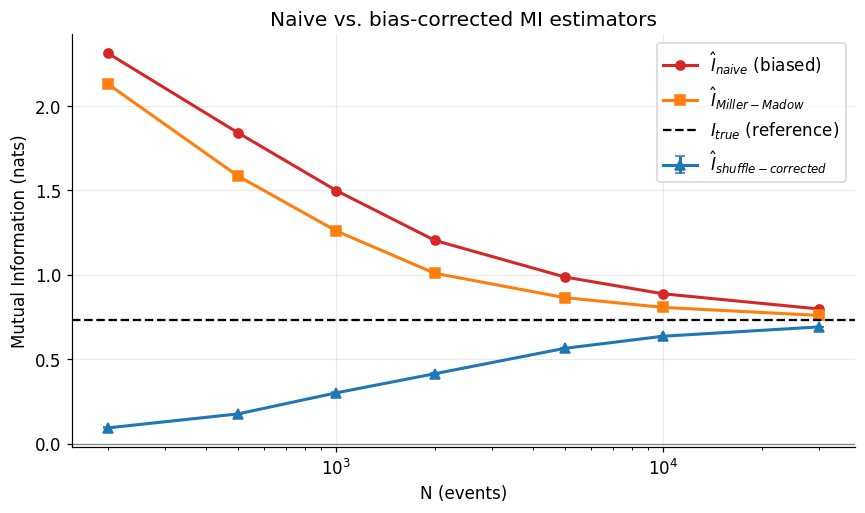
\includegraphics[width=0.75\textwidth]{figs/fig04_naive_vs_corrected.png}
\caption{Naive vs.\ bias-corrected MI estimators across sample sizes.}
\label{fig:naive-vs-corrected}
\end{figure}

\begin{figure}[htb]
\centering
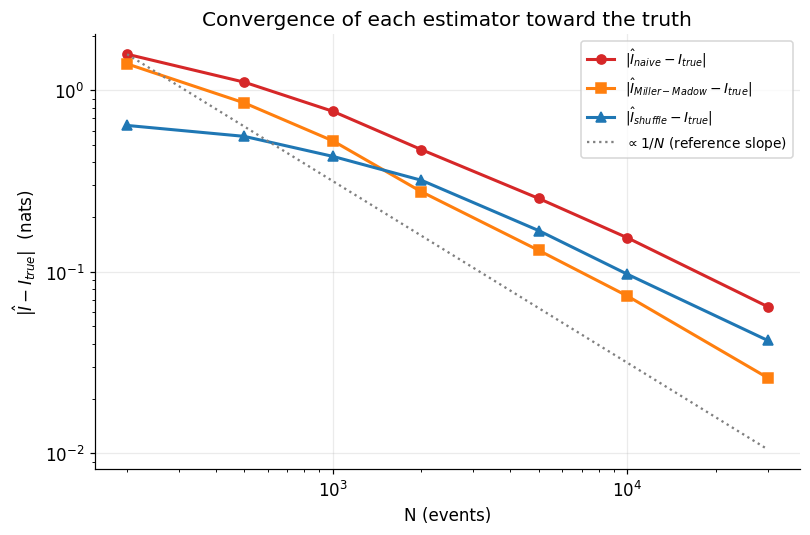
\includegraphics[width=0.75\textwidth]{figs/fig05_residual_convergence.png}
\caption{Convergence of each estimator toward the true value, on a log-log
scale, with a $1/N$ reference slope.}
\label{fig:residuals}
\end{figure}

% =============================================================================
\section{The rigorous fix: NSB Bayesian entropy estimator}
\label{sec:nsb}
% =============================================================================

Both corrections above are still, fundamentally, \textbf{point corrections
derived under a large-$N$ assumption} -- they estimate one number (the
bias) and subtract it. The \textbf{Nemenman--Shafee--Bialek (NSB)}
estimator takes a genuinely different approach: instead of correcting a
biased point estimate, it computes the \textbf{Bayesian posterior mean
entropy} directly, using a prior specifically constructed to avoid
smuggling in any implicit assumption about how spread-out the distribution
is. This is the standard tool for the severely-undersampled regime
($N\lesssim K$) in the neuroscience spike-train MI literature -- precisely
our regime once hadron multiplicities are binned in 2D.

The construction, in four steps:

\begin{enumerate}
\item Put a symmetric Dirichlet prior $P(p\,|\,\beta)\propto\prod_i
p_i^{\beta-1}$ over the $K$ possible bin probabilities. For any fixed
$\beta$, the posterior mean entropy given counts $\{n_i\}$ has a closed
form,
\begin{equation}
\langle S\rangle_{\beta,n} = \psi_0(N+K\beta+1) -
\sum_i \frac{n_i+\beta}{N+K\beta}\,\psi_0(n_i+\beta+1).
\end{equation}

\item \textbf{The catch:} a flat prior on $\beta$ does \emph{not} give a
flat prior on entropy -- for large $K$, $P(S\,|\,\beta)$ is sharply peaked
as a function of $\beta$. Fixing any single $\beta$ (as ordinary
add-one/Laplace/Jeffreys smoothing does) silently assumes an entropy value
before looking at the data.

\item NSB's fix: reweight $\beta$ by the hyperprior that makes the
\emph{induced} prior on $S$ flat -- literally the rate of change of the
prior mean entropy with $\beta$,
\begin{equation}
\rho(\beta) = K\,\psi_1(K\beta+1) - \psi_1(\beta+1).
\end{equation}

\item Average over $\beta$, weighted by both this hyperprior and the
Dirichlet--multinomial evidence $P(n\,|\,\beta)$,
\begin{equation}
\hat S_{\rm NSB} =
\frac{\int_0^\infty d\beta\;\rho(\beta)\,P(n\,|\,\beta)\,\langle
S\rangle_{\beta,n}}
{\int_0^\infty d\beta\;\rho(\beta)\,P(n\,|\,\beta)}.
\end{equation}
\end{enumerate}

This reduces to a tractable 1D numerical integral. We apply it separately
to $S_A,S_B,S_{AB}$ (each needs its own alphabet size $K$: for the joint
distribution, $K_{AB}^{\rm alphabet}=K_A^{\rm alphabet}\times K_B^{\rm
alphabet}$, the full product space of possible outcomes -- not the
observed $K_{AB}$ count from before, since NSB needs to know the size of
the space being integrated over, not how much of it happened to be hit),
then combine: $\hat I_{\rm NSB} = \hat S_A^{\rm NSB}+\hat S_B^{\rm
NSB}-\hat S_{AB}^{\rm NSB}$.

\begin{table}[h]
\centering
\caption{All four MI estimators, head to head.}
\begin{tabular}{rrrrrr}
\toprule
$N$ & $\hat I_{\rm naive}$ & $\hat I_{MM}$ & $\hat I_{\rm shuffle}$ &
$\hat I_{\rm NSB}$ & $\Itrue$ (ref.) \\
\midrule
200   & 2.3511 & 2.1711 & 0.0578 & 0.5098 & 0.7329 \\
500   & 1.7525 & 1.5035 & 0.2137 & 0.6833 & 0.7329 \\
1000  & 1.5071 & 1.2711 & 0.3062 & 0.7369 & 0.7329 \\
2000  & 1.2299 & 1.0367 & 0.4340 & 0.7416 & 0.7329 \\
5000  & 1.0030 & 0.8842 & 0.5807 & 0.7678 & 0.7329 \\
20000 & 0.8222 & 0.7716 & 0.6752 & 0.7411 & 0.7329 \\
\bottomrule
\end{tabular}
\end{table}

NSB tracks $\Itrue$ closely across the entire range, including at
$N=200$ where the naive estimator is off by roughly a factor of three and
Miller--Madow has barely moved. This is the payoff of treating the whole
problem as Bayesian inference over entropy rather than patching a biased
point estimate after the fact. Figure~\ref{fig:nsb-comparison} adds NSB to
the convergence comparison: its residual curve sits visibly below the
other three methods across most of the range, and in particular stays far
more stable at small $N$ -- it doesn't need $N\gg K$ to behave sensibly.

\begin{figure}[htb]
\centering
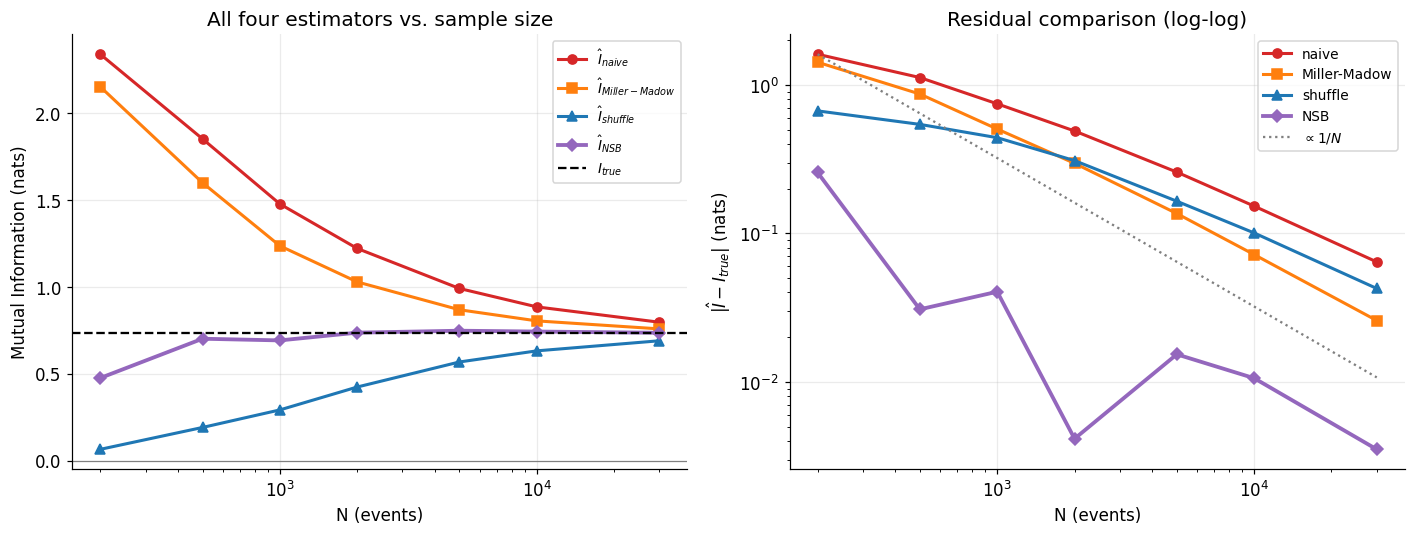
\includegraphics[width=\textwidth]{figs/fig06_nsb_comparison.png}
\caption{Left: all four estimators vs.\ sample size. Right: residual
comparison on a log-log scale, with a $1/N$ reference slope.}
\label{fig:nsb-comparison}
\end{figure}

\paragraph{Practical notes for the real STAR dijet data.}
\begin{itemize}
\item The alphabet size $K$ (for each marginal, and $K_A\times K_B$ for
the joint) needs to be fixed \emph{before} looking at the data -- pick a
generous fixed upper bound on plausible hadron multiplicity per jet
(e.g.\ from detector acceptance / kinematic limits), not the observed
range, or a data-dependent bias is reintroduced through the back door.
\item NSB is somewhat more expensive per call than MM or
shuffle-subtraction (a 1D numerical integral instead of a closed-form
correction or a handful of permutations), but it remains a fraction of a
second per event sample -- entirely practical for a real analysis,
including a full jackknife or bootstrap for uncertainty quantification.
\item The same estimator applies directly to $\SBA=S_{AB}-S_A$ -- swap in
the NSB entropies there instead of the naive/MM/shuffle versions before
making any negative-conditional-entropy (quantum) claim, as done next.
\end{itemize}

% =============================================================================
\section{Putting it together: quantum-signal detection sensitivity}
\label{sec:sensitivity}
% =============================================================================

Section~\ref{sec:observable} established $\SBA=S_{AB}-S_A$ as the correct,
computable witness (provably $\geq0$ classically), and
Secs.~\ref{sec:bias}--\ref{sec:nsb} established that NSB is the
best-behaved bias-corrected estimator, especially at small $N$. Here we
combine both: since our toy model is itself purely classical, its true
$\SBA$ is a known, solidly positive number ($\SBA_{\rm true}=3.1524$
nats) -- exactly the right sandbox to measure the \textbf{statistical
noise floor} of the NSB estimator against a known ground truth, and turn
that into a quantitative statement about how large a genuine quantum
excess would need to be, at a given event count, to be distinguishable
from this noise floor.

\textbf{Design:} for a grid of $N$, we draw many independent samples from
the same generative model, compute $\hat S(B|A)_{\rm NSB}$ for each, and
take the spread over draws as the estimator's sampling uncertainty
$\sigma_{\rm NSB}(N)$ at that statistics. A hypothetical genuine quantum
excess of magnitude $\Delta$ is then detectable at $z$ standard
deviations once
\begin{equation}
\Delta \;>\; z\,\sigma_{\rm NSB}(N).
\end{equation}
Equivalently, the \textbf{minimum detectable quantum signal} at a chosen
confidence level ($z=3$, a common ``solid evidence'' threshold, used
below) is $\Delta_{\rm min}(N)=z\,\sigma_{\rm NSB}(N)$. In a real analysis
with one actual dataset -- not a synthetic model with known truth --
$\sigma_{\rm NSB}(N)$ would be estimated directly from that dataset via
bootstrap or jackknife resampling, rather than from independent Monte
Carlo replicates as done here for demonstration.

Figure~\ref{fig:noise-floor} shows the NSB (and, for comparison, naive and
Miller--Madow) estimates of $\SBA$ vs.\ $N$, together with their
sampling standard deviation. NSB has both the smallest bias (its mean
tracks $\SBA_{\rm true}$ most closely, especially at small $N$) and a
noise floor that shrinks cleanly with $N$, following the expected
$1/\sqrt{N}$ statistical scaling.

\begin{figure}[htb]
\centering
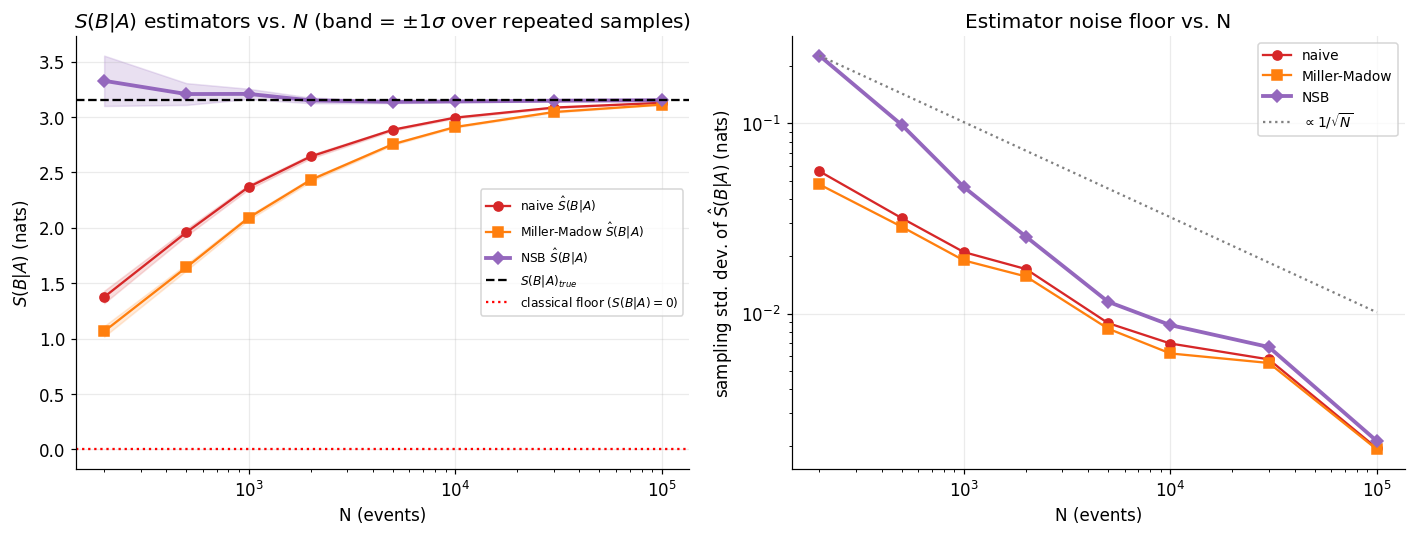
\includegraphics[width=\textwidth]{figs/fig07_sba_noise_floor.png}
\caption{Left: $\SBA$ estimators vs.\ $N$ (bands: $\pm1\sigma$ over
repeated samples). Right: sampling standard deviation of each estimator
vs.\ $N$, with a $1/\sqrt{N}$ reference slope.}
\label{fig:noise-floor}
\end{figure}

Converting the NSB noise floor into a minimum-detectable-signal curve
(Fig.~\ref{fig:detection-sensitivity}) and fitting a power law gives a
direct, quantitative answer to ``how big must a quantum signal be, at a
given statistics, to be believable'':

\begin{table}[h]
\centering
\caption{Minimum event count $N$ needed for a $3\sigma$ detection of a
hypothetical quantum-correlation excess of the given magnitude, from the
fitted $\Delta_{\rm min}(N)\propto N^{-0.72}$ power law.}
\begin{tabular}{rr}
\toprule
Assumed $|\SBA_{\rm quantum}|$ (nats) & $N$ needed for $3\sigma$ detection \\
\midrule
0.500 & 201 \\
0.200 & 722 \\
0.100 & 1{,}899 \\
0.050 & 4{,}995 \\
0.020 & 17{,}934 \\
0.010 & 47{,}164 \\
\bottomrule
\end{tabular}
\end{table}

\begin{figure}[htb]
\centering
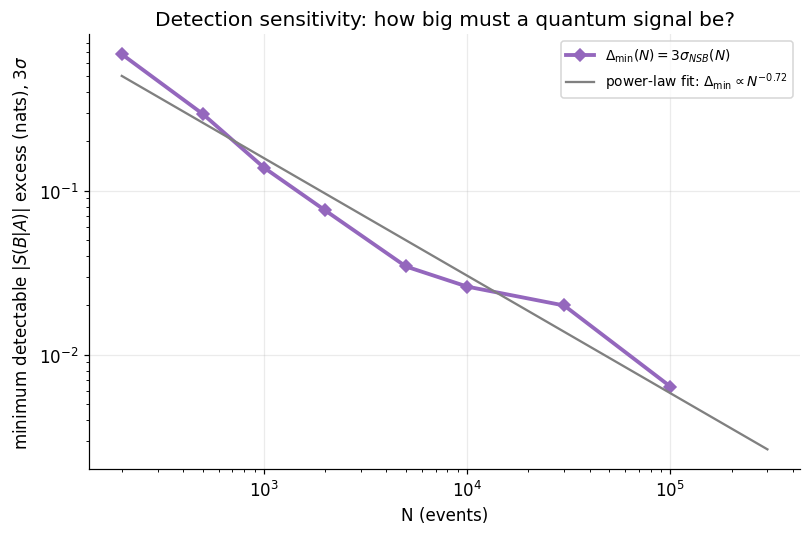
\includegraphics[width=0.75\textwidth]{figs/fig08_detection_sensitivity.png}
\caption{Minimum detectable $|\SBA|$ excess at $3\sigma$, vs.\ event
count $N$, with a power-law fit for interpolation/extrapolation.}
\label{fig:detection-sensitivity}
\end{figure}

\paragraph{Caveats to carry into the real analysis.}
\begin{itemize}
\item $\sigma_{\rm NSB}(N)$ here is measured \emph{at the true classical
value} ($\SBA_{\rm true}\approx$ a few nats for our toy correlation
strength), not at the boundary $\SBA=0$. Entropy-estimator variance
depends on the shape of the underlying distribution, not just $N$, so the
true noise floor near a genuinely small or slightly-negative $\SBA$ could
differ somewhat from this estimate. For the real STAR data, this bootstrap
procedure should be re-run centered on the actual observed operating point
(via jackknife/bootstrap on the real dataset itself), rather than trusting
this toy-model number directly.
\item This procedure characterizes sensitivity to a violation of the
classical conditional-entropy bound using multiplicity data alone
(Sec.~\ref{sec:observable}). It is not a substitute for an actual quantum
witness such as a Bell/CHSH inequality on the $\Lambda\bar\Lambda$ spin
observables, which remains the model-independent way to certify
entanglement rather than merely rule out one particular classical
description.
\end{itemize}

% =============================================================================
\section{Summary and recommendations from the toy Monte Carlo study}
% =============================================================================

\begin{enumerate}

\item \textbf{The correct witness} is $\SBA=S_{AB}-S_A$ (and $S(A|B)$,
check both directions), which must be $\geq0$ for any classical
distribution. Genuine quantum discord (Ollivier--Zurek) cannot be
computed from hadron-count histograms alone -- any classical joint
distribution trivially gives discord $=0$; it would require actual
quantum-state tomography (e.g.\ the $\Lambda\bar\Lambda$
spin-density-matrix channel).

\item \textbf{The naive plug-in MI estimator is always biased upward},
with leading term $\approx(K_{AB}-K_A-K_B+1)/(2N)$. Coarser binning or
fewer events both make it worse -- comparing different STAR running
periods, luminosities, or binning choices will report different central
MI values from what should be the same physics, purely from this effect.

\item \textbf{Miller--Madow} (done correctly, using the observed
$K_{AB}$, not the product $K_AK_B$) and \textbf{shuffle-subtraction} both
substantially reduce this bias and stay well-behaved, but neither is exact
at small $N$: Miller--Madow is a first-order truncation;
shuffle-subtraction tends to systematically overcorrect when the true
correlation is strong.

\item \textbf{NSB} is the recommended estimator for the real analysis: a
Bayesian posterior-mean entropy built on a prior specifically constructed
to be uninformative about entropy itself. It tracks the truth closely
across the entire tested $N$ range, including deep in the
severely-undersampled regime where the other methods struggle, at a
modest computational cost.

\item \textbf{Before claiming any quantum-correlation excess}, bias-correct
with NSB and compare against the estimator's own sampling noise floor at
that $N$ (bootstrapped from the real dataset via jackknife/bootstrap, not
assumed from this toy model). Section~\ref{sec:sensitivity} works this out
quantitatively: the NSB noise floor shrinks $\propto 1/\sqrt{N}$, giving a
concrete minimum-detectable-signal curve
$\Delta_{\rm min}(N)=z\,\sigma_{\rm NSB}(N)$ -- a direct, quotable answer
to ``how big must a genuine quantum excess be, at a given event count, to
be distinguishable from finite-sample bias and noise.''

\item \textbf{This entire procedure only tests a violation of the
classical conditional-entropy bound.} It is a necessary check before any
stronger quantum claim, but is not itself a model-independent entanglement
certification -- that role is played by the Bell/CHSH-type inequality on
spin observables in the parallel $\Lambda\bar\Lambda$ program.

\end{enumerate}

% =============================================================================
\section{Validation on PYTHIA~8 Monte Carlo simulation}
\label{sec:pythia}
% =============================================================================

The toy model of Secs.~\ref{sec:toymc}--\ref{sec:nsb} demonstrates that the
estimator pipeline behaves correctly on data with a known, simple
generative structure. The natural next step is to check the same pipeline
on a full QCD event generator, where hadron multiplicities arise from
parton showering, hadronization, and (optionally) the underlying event --
none of which was built into the toy model by hand. We generated
back-to-back charged-jet dijets with PYTHIA~8 (Monash 2013 tune,
anti-$k_T$ jets, $R=0.4$, charged final-state particles only, matching a
STAR-TPC-like charged-jet definition) and applied the identical naive/
Miller--Madow/shuffle/NSB pipeline, unmodified, to the generator output.

This particular validation run used LHC-like kinematics
($\sqrt{s}=14$~TeV rather than the $\sqrt{s}=200$~GeV RHIC energy that
motivates the eventual STAR measurement) specifically \emph{because} of
its much wider accessible jet-$p_T$ range: as discussed below
(Sec.~\ref{sec:pythia-ptdep}), the multiplicity-vs-$p_T$ correlation
predicted by QCD is intrinsically a slow, logarithmic effect, and a wide
dynamic range makes it far easier to confirm the pipeline is tracking real
physics rather than an artifact of a narrow kinematic window. The $200$~GeV
run for the actual STAR measurement is a separate, ongoing exercise (see
Sec.~\ref{sec:conclusions}); everything in this section is a
\emph{methods validation}, not a physics result.

\subsection{Multiplicity and $p_T$ distributions}

Figure~\ref{fig:py-mult-dist} shows the charged-multiplicity distributions
for the leading and subleading jets, overlaid with a method-of-moments
Negative-Binomial fit (as in Sec.~\ref{sec:toymc}). Both jets show genuine
overdispersion relative to Poisson (var/mean $=1.55$ for the leading jet,
$1.29$ for the subleading jet), qualitatively consistent with -- though
not identical in shape to -- the NBD-like multiplicity distributions
assumed in the toy model. This is a useful cross-check in its own right:
the toy model's central structural assumption (NBD-shaped marginals) is
not merely a convenient fiction, but a reasonable approximation to what a
full QCD generator actually produces.

\begin{figure}[htb]
\centering
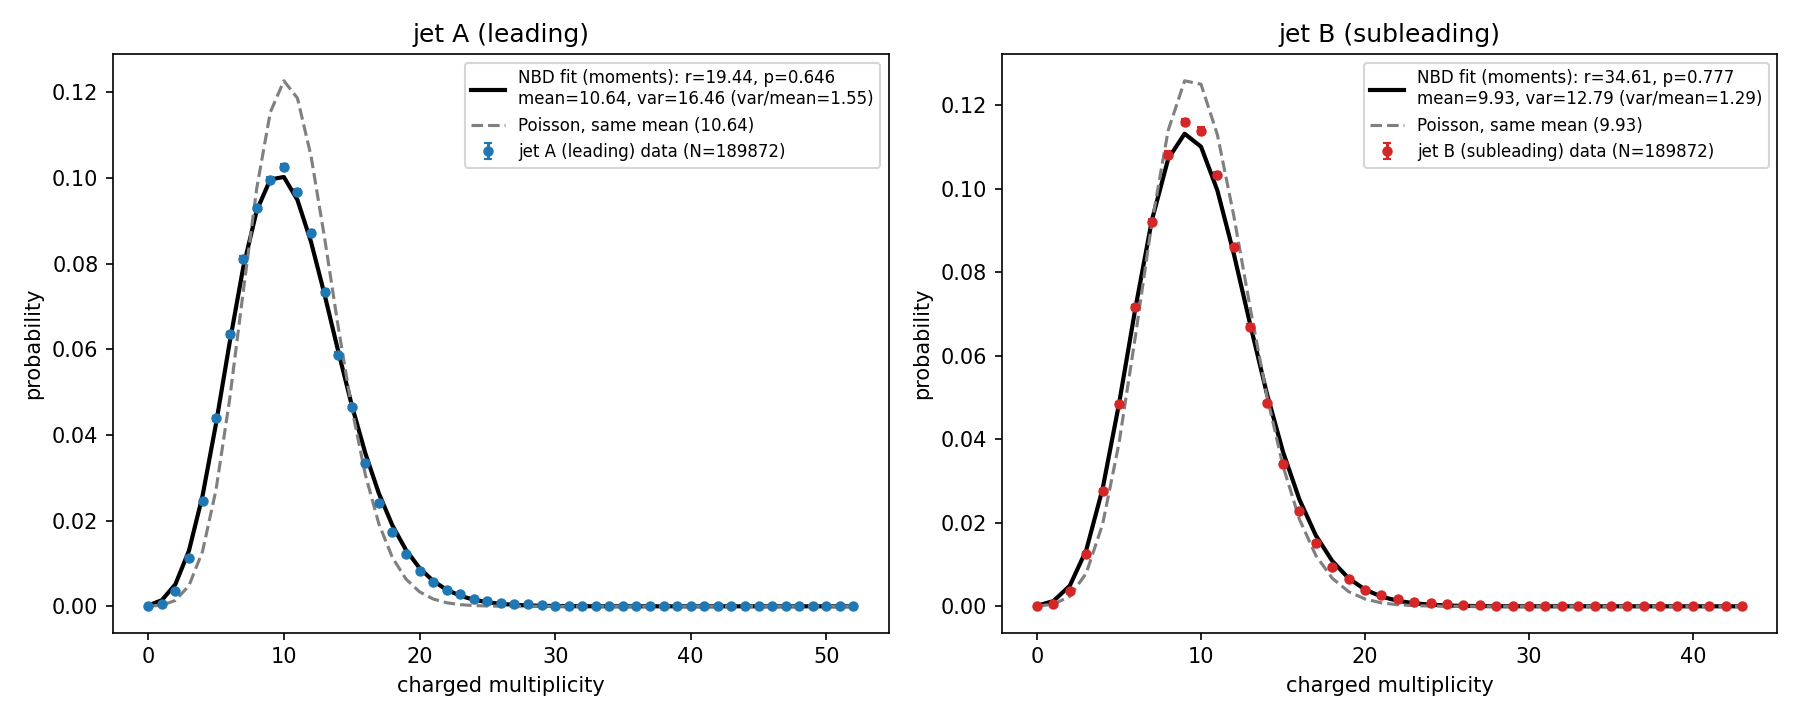
\includegraphics[width=\textwidth]{figs/dijet_entropy_result_truth_multiplicity_dists.png}
\caption{PYTHIA~8: charged-multiplicity distributions for the leading
(left) and subleading (right) jet, with NBD and same-mean Poisson overlay
(cf.\ the toy-model version, Sec.~\ref{sec:toymc}).}
\label{fig:py-mult-dist}
\end{figure}

Figure~\ref{fig:py-joint-mult} shows the corresponding joint distribution:
36.9\% of the $53\times44$ grid is occupied ($K_{AB}=861$) at
$N\approx1.9\times10^5$ events -- a moderately, not severely, undersampled
regime, comparable to the middle of the range explored in the toy study.
Figure~\ref{fig:py-pt-dist} shows the (steeply falling, as expected for a
QCD jet spectrum) leading- and subleading-jet $p_T$ distributions, and
Fig.~\ref{fig:py-joint-pt} their joint distribution -- the latter makes
visually clear why quantile (rather than fixed-width) $p_T$ binning is
necessary for the differential measurements below: the bulk of events sit
in a narrow low-$p_T$ band, with a long, sparse tail.

\begin{figure}[htb]
\centering
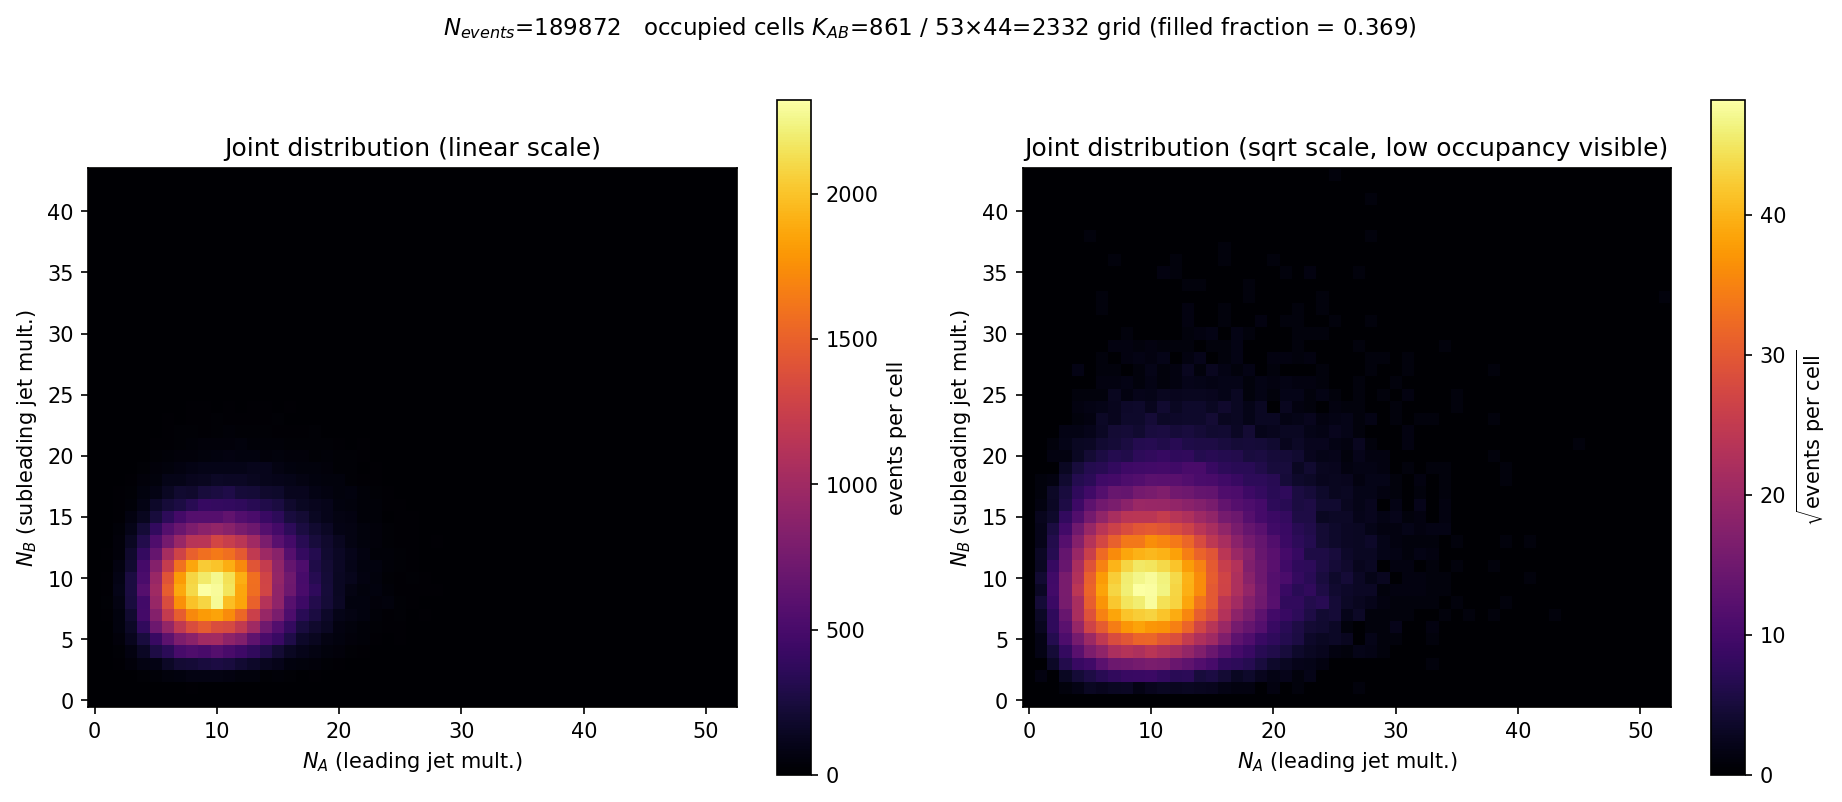
\includegraphics[width=0.85\textwidth]{figs/dijet_entropy_result_truth_joint_multiplicity_dist.png}
\caption{PYTHIA~8: joint charged-multiplicity distribution, linear and
sqrt color scale (cf.\ Fig.~\ref{fig:marginals-joint}).}
\label{fig:py-joint-mult}
\end{figure}

\begin{figure}[htb]
\centering
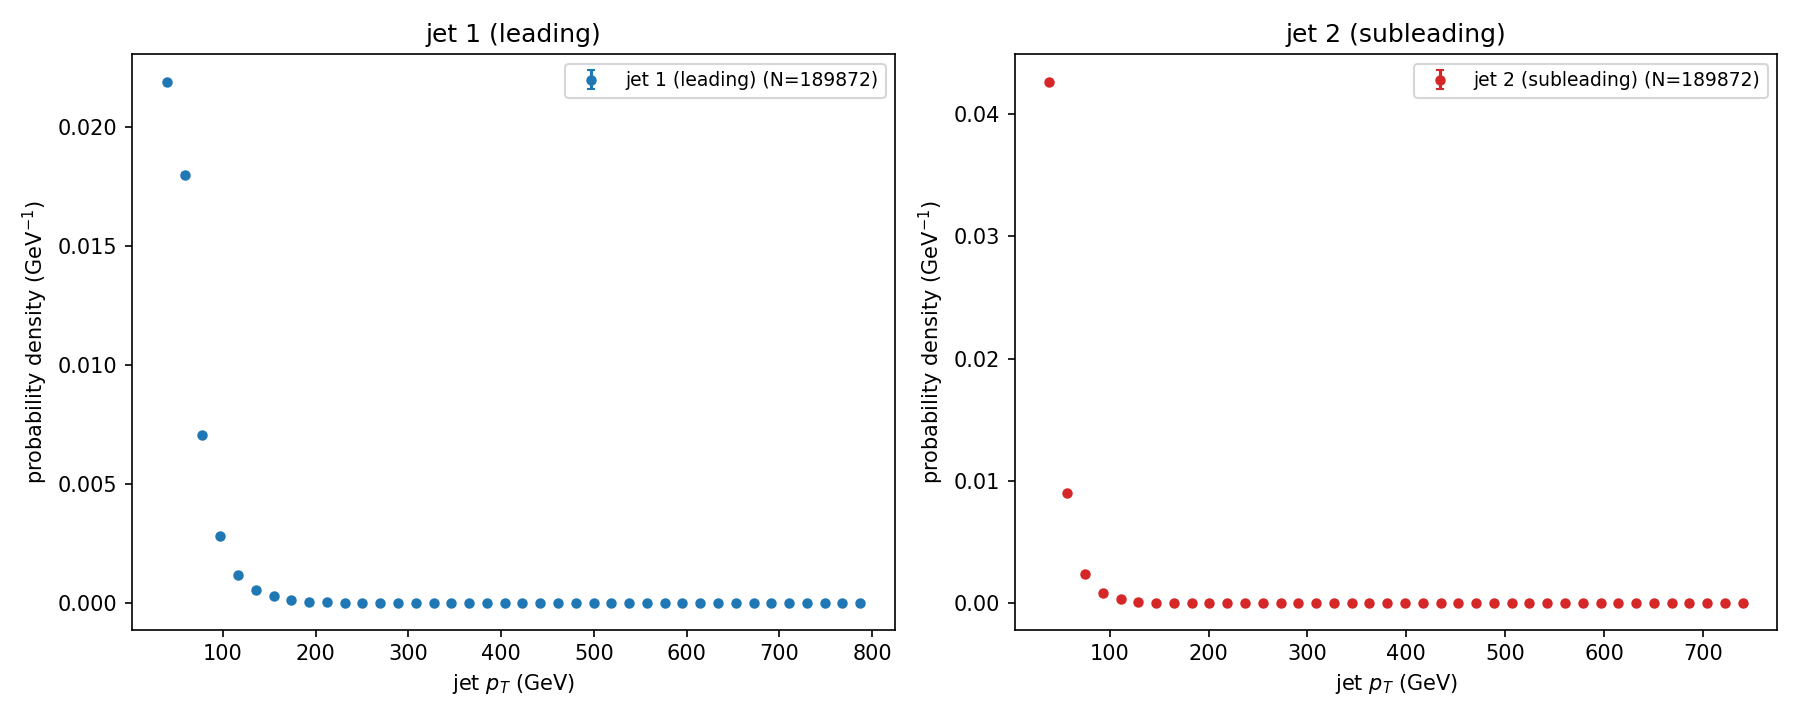
\includegraphics[width=\textwidth]{figs/dijet_entropy_result_truth_pt_dists.png}
\caption{PYTHIA~8: leading- and subleading-jet $p_T$ distributions.}
\label{fig:py-pt-dist}
\end{figure}

\begin{figure}[htb]
\centering
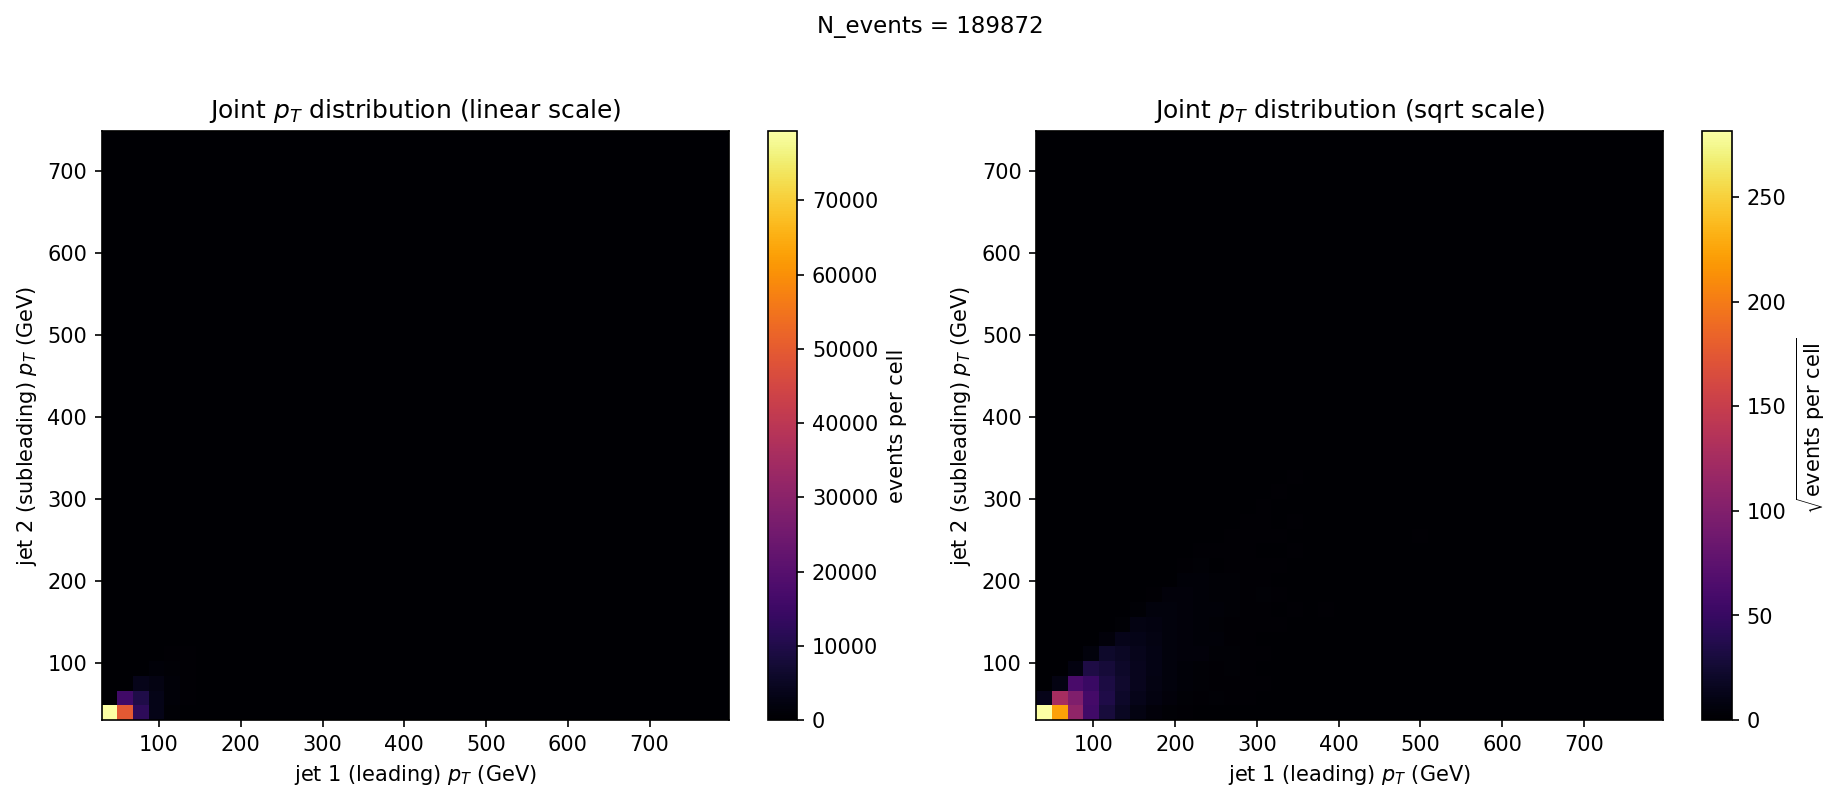
\includegraphics[width=0.85\textwidth]{figs/dijet_entropy_result_truth_joint_pt_dist.png}
\caption{PYTHIA~8: joint leading/subleading jet $p_T$ distribution,
linear and sqrt color scale.}
\label{fig:py-joint-pt}
\end{figure}

\subsection{The multiplicity--$p_T$ correlation}
\label{sec:pythia-ptdep}

A basic physical expectation -- confirmed experimentally (e.g.\ ALICE,
arXiv:2311.13322: ``the mean charged-particle multiplicity inside the
leading jet cone rises monotonically with increasing jet $p_T$'') -- is
that higher-$p_T$ jets should carry higher charged multiplicity, via
additional phase space for parton radiation before hadronization. This
growth is predicted by QCD coherent-branching (MLLA) arguments to be slow
and roughly \emph{logarithmic} in $p_T$, not linear, which matters
directly for how easy the effect is to see over a limited kinematic range
(as it was, initially, in an earlier $200$~GeV validation attempt with a
narrower accessible $p_T$ window).

Figure~\ref{fig:py-mult-vs-pt} shows the raw, unbinned-by-any-entropy-
machinery profile of mean charged multiplicity vs.\ jet $p_T$, together
with a weighted fit of the MLLA-motivated form $\langle N\rangle = a +
b\ln p_T$. The fitted slope is highly significant for both jets ($b =
3.77\pm0.05$, $83\sigma$, leading jet; $b=4.71\pm0.07$, $66\sigma$,
subleading jet) -- direct, quantitative confirmation that PYTHIA~8
reproduces the expected QCD multiplicity-growth pattern, and that the
analysis pipeline correctly recovers it from generator output with no
prior assumption beyond bin means and standard errors.

\begin{figure}[htb]
\centering
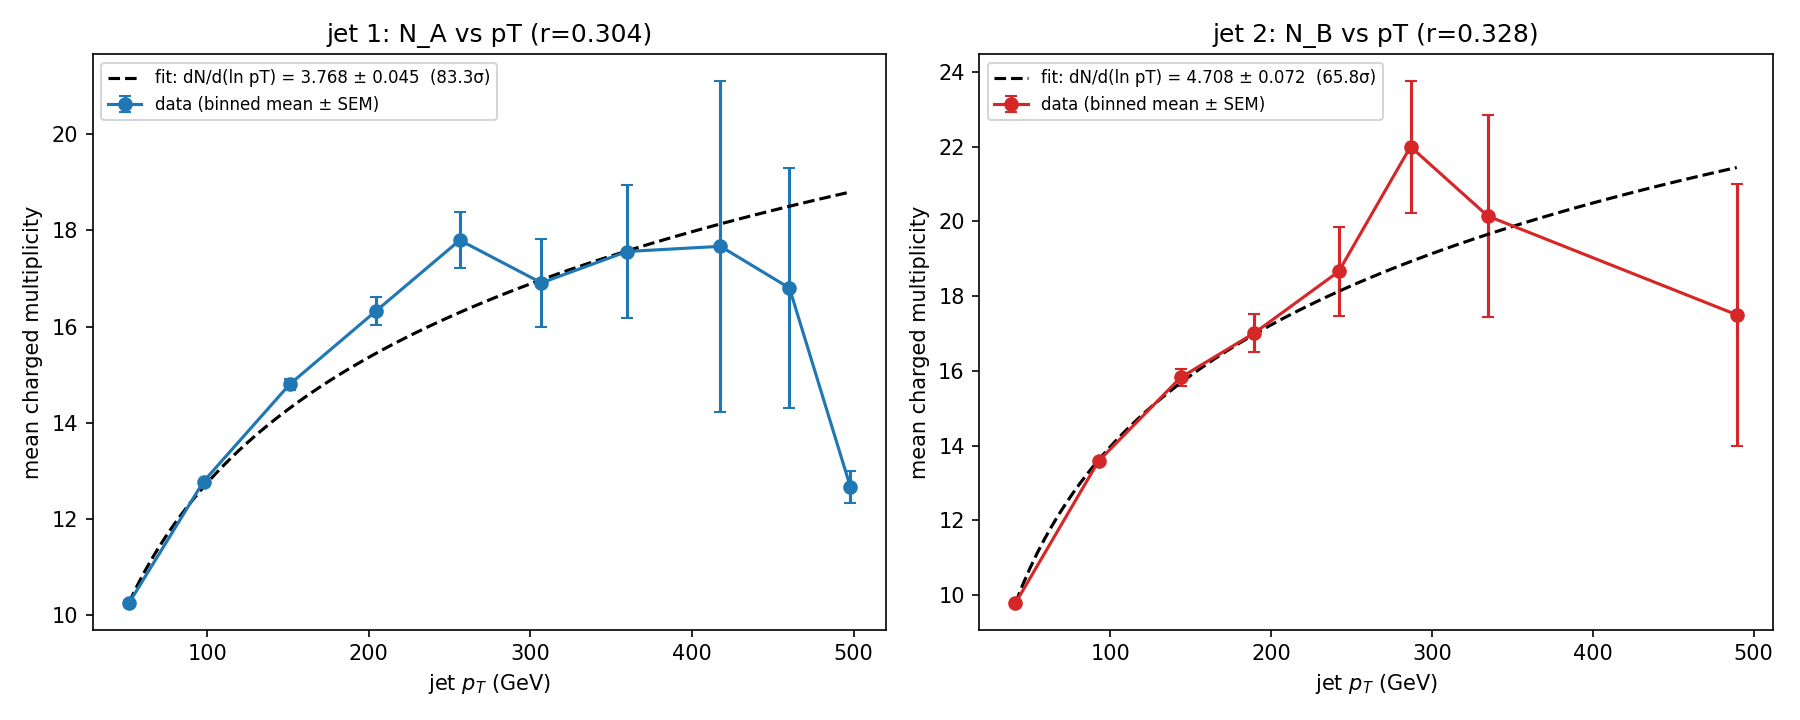
\includegraphics[width=\textwidth]{figs/dijet_entropy_result_truth_mult_vs_pt_profile.png}
\caption{PYTHIA~8: raw mean charged multiplicity vs.\ jet $p_T$ (binned
mean $\pm$ SEM), with a weighted fit to $\langle N\rangle=a+b\ln p_T$.
Both slopes are significant at $>60\sigma$.}
\label{fig:py-mult-vs-pt}
\end{figure}

\subsection{Finite-sample bias, reproduced on generator output}

Figure~\ref{fig:py-bias-scan} repeats the toy study's core diagnostic
(Sec.~\ref{sec:toymc}) directly on subsamples of the real PYTHIA~8 output:
the naive $\hat I$ falls from $\approx0.66$~nats at $N=200$ down toward
the full-sample NSB value ($\approx0.009$~nats) as $N$ grows to
$\approx1.9\times10^5$ -- the same qualitative bias curve seen throughout
Sec.~\ref{sec:toymc}, now confirmed on a dataset the toy model was never
built to resemble. This is a meaningful cross-check: the bias mechanism
identified analytically (Sec.~\ref{sec:bias}) and demonstrated on a
synthetic Gamma-Poisson model is not an artifact of that specific
generative structure -- it appears with the same shape on genuine QCD
Monte Carlo output.

\begin{figure}[htb]
\centering

\includegraphics[width=0.8\textwidth]{figs/dijet_entropy_result_truth_bias_scan.png}
\caption{PYTHIA~8: naive $\hat I$ vs.\ subsample size $N$, real generator
output (cf.\ the toy-model version, Fig.~\ref{fig:bias-vs-N}).}
\label{fig:py-bias-scan}
\end{figure}

\subsection{Point estimates on the full sample}

Figure~\ref{fig:py-summary} shows all four estimators on the full sample
($N\approx1.9\times10^5$): naive ($0.0112\pm0.0004$), Miller--Madow
($0.0092\pm0.0004$), shuffle-corrected ($0.0084\pm0.0003$), and NSB
($0.0085\pm0.0004$~nats) -- naive sits visibly above the other three, as
expected from the bias mechanism above, while Miller--Madow/shuffle/NSB
agree closely with each other, consistent with all three having converged
toward the true value at this statistics (matching the closure seen among
independently-biased estimators at large $N$ in the toy study,
Sec.~\ref{sec:toymc}). The conditional entropy $\SBA=2.65$~nats sits far
above the classical floor, with no indication of a quantum violation --
expected and unsurprising, since PYTHIA~8 is itself a classical
event-by-event simulator with no entanglement built into its hadronization
model. This measurement is a validation of the estimator machinery, not a
physics claim; the analogous measurement on real detector data is where a
genuine quantum question would be asked.

\begin{figure}[htb]
\centering
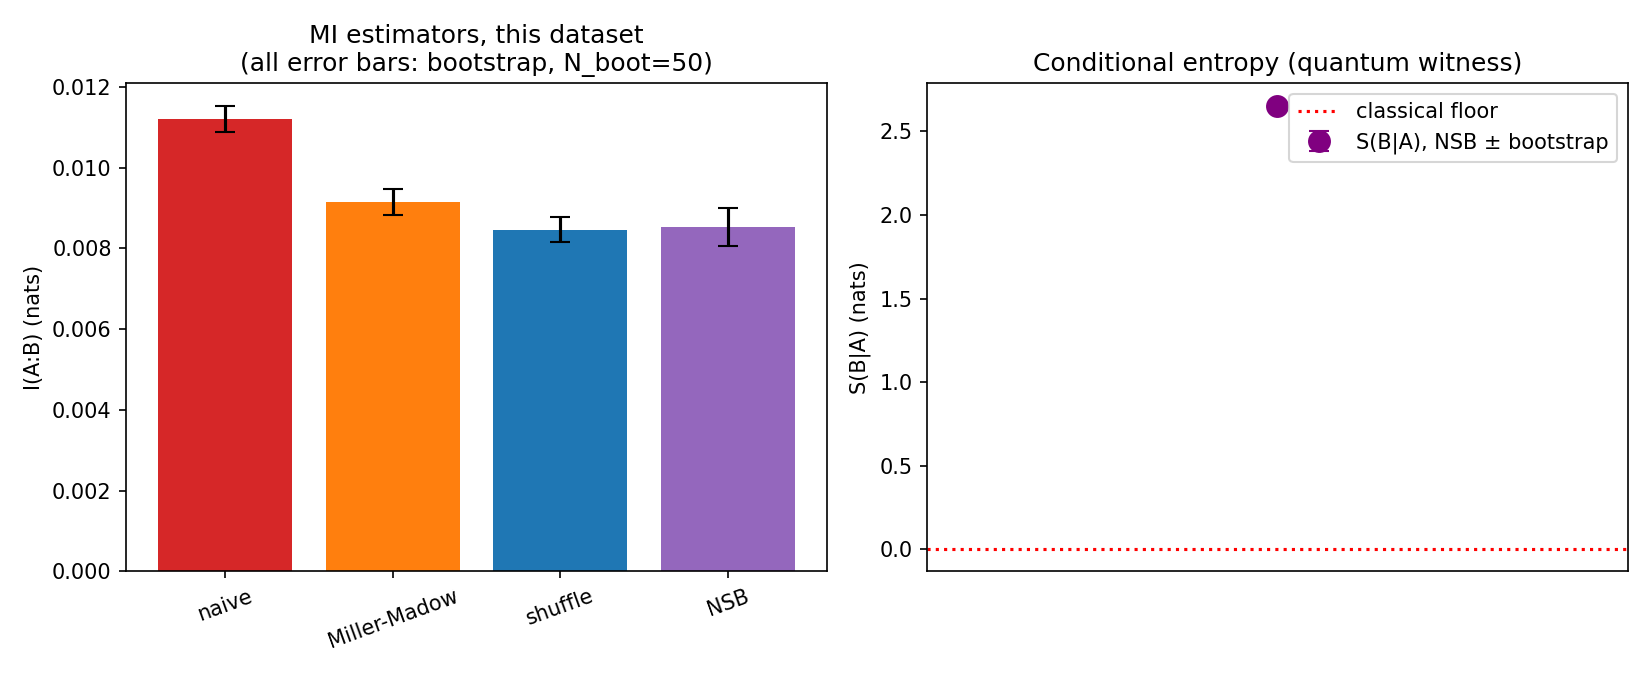
\includegraphics[width=\textwidth]{figs/dijet_entropy_result_truth_summary.png}
\caption{PYTHIA~8: all four MI estimators (left) and $\SBA$ (right) on
the full sample, bootstrap error bars.}
\label{fig:py-summary}
\end{figure}

\subsection{Differential measurement vs.\ jet $p_T$}

Figures~\ref{fig:py-entropy-pt}--\ref{fig:py-sba-pt} show $S_A,S_B,S_{AB}$,
$I(A{:}B)$, and $\SBA$ (NSB) in quantile bins of leading-jet $p_T$. All
three entropies rise smoothly with $p_T$ (Fig.~\ref{fig:py-entropy-pt}),
directly reflecting the multiplicity growth of Sec.~\ref{sec:pythia-ptdep}.
$I(A{:}B)$ (Fig.~\ref{fig:py-mi-pt}) also rises with $p_T$, modestly at
low-to-mid $p_T$ and more sharply in the highest (widest, most
statistics-limited) bin; $\SBA$ (Fig.~\ref{fig:py-sba-pt}) stays solidly
positive and rising throughout, consistent with a classical description at
every $p_T$ probed.

\begin{figure}[htb]
\centering
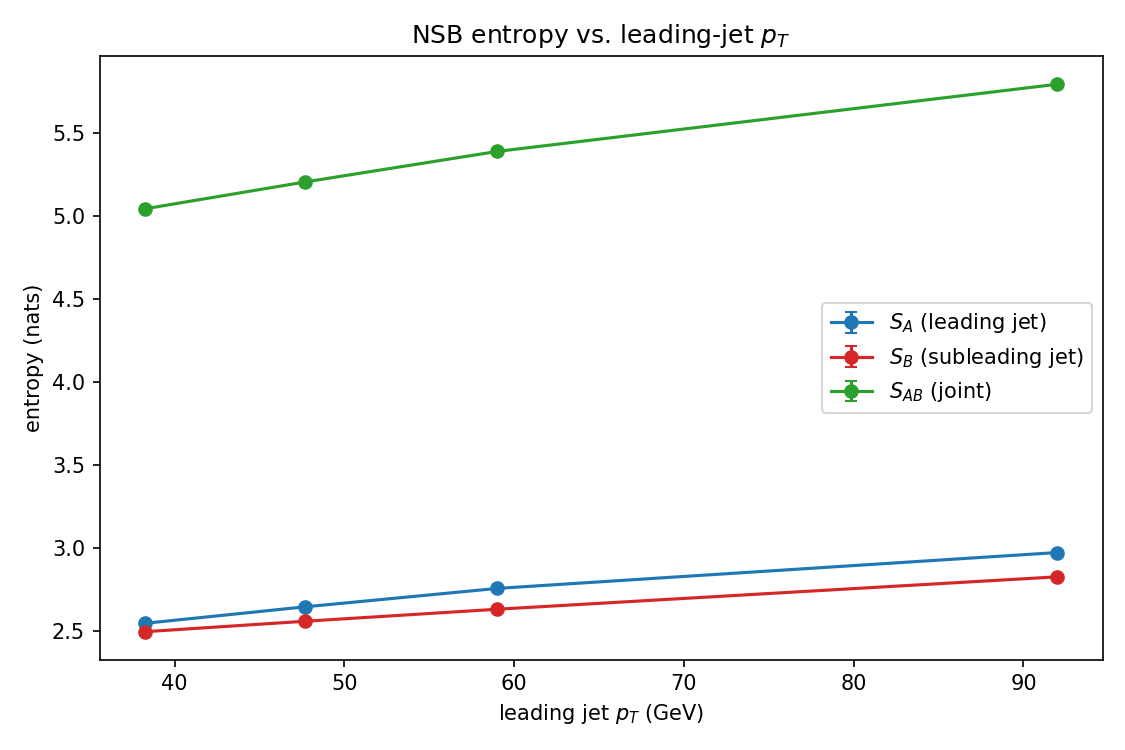
\includegraphics[width=\textwidth]{figs/dijet_entropy_result_truth_entropy_vs_pt.png}
\caption{PYTHIA~8: $S_A,S_B,S_{AB}$ (NSB) vs.\ leading-jet $p_T$.}
\label{fig:py-entropy-pt}
\end{figure}

\begin{figure}[htb]
\centering
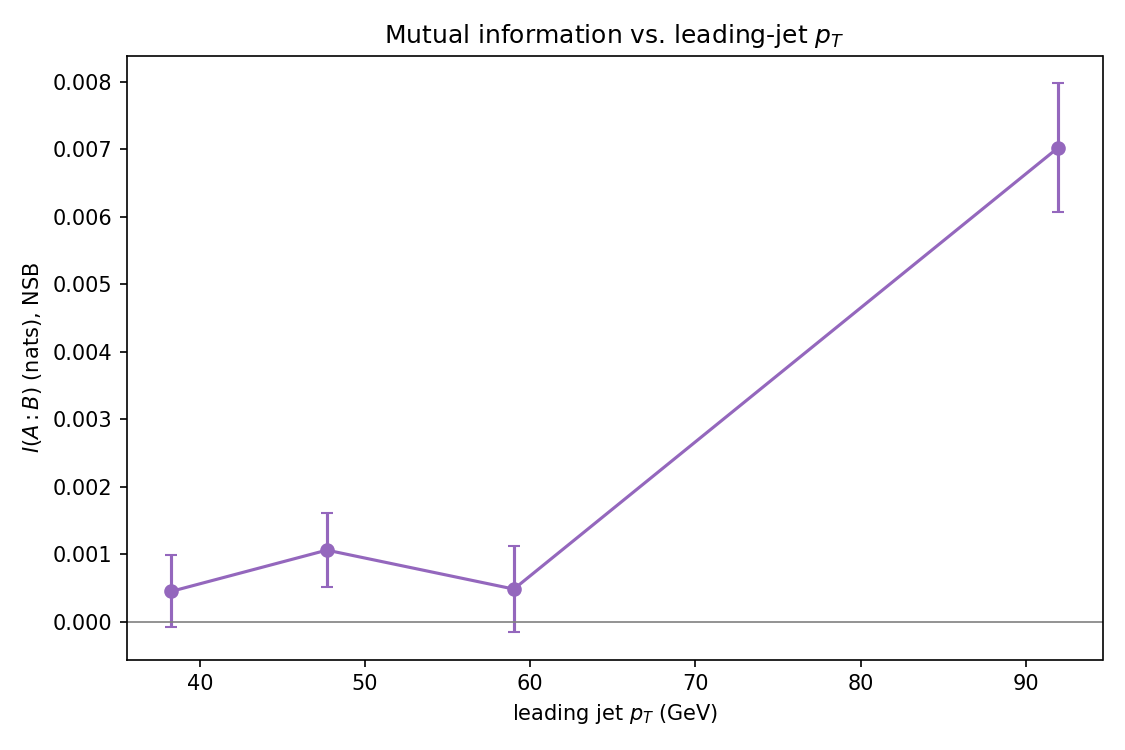
\includegraphics[width=0.8\textwidth]{figs/dijet_entropy_result_truth_MI_vs_pt.png}
\caption{PYTHIA~8: $I(A{:}B)$ (NSB) vs.\ leading-jet $p_T$.}
\label{fig:py-mi-pt}
\end{figure}

\begin{figure}[htb]
\centering
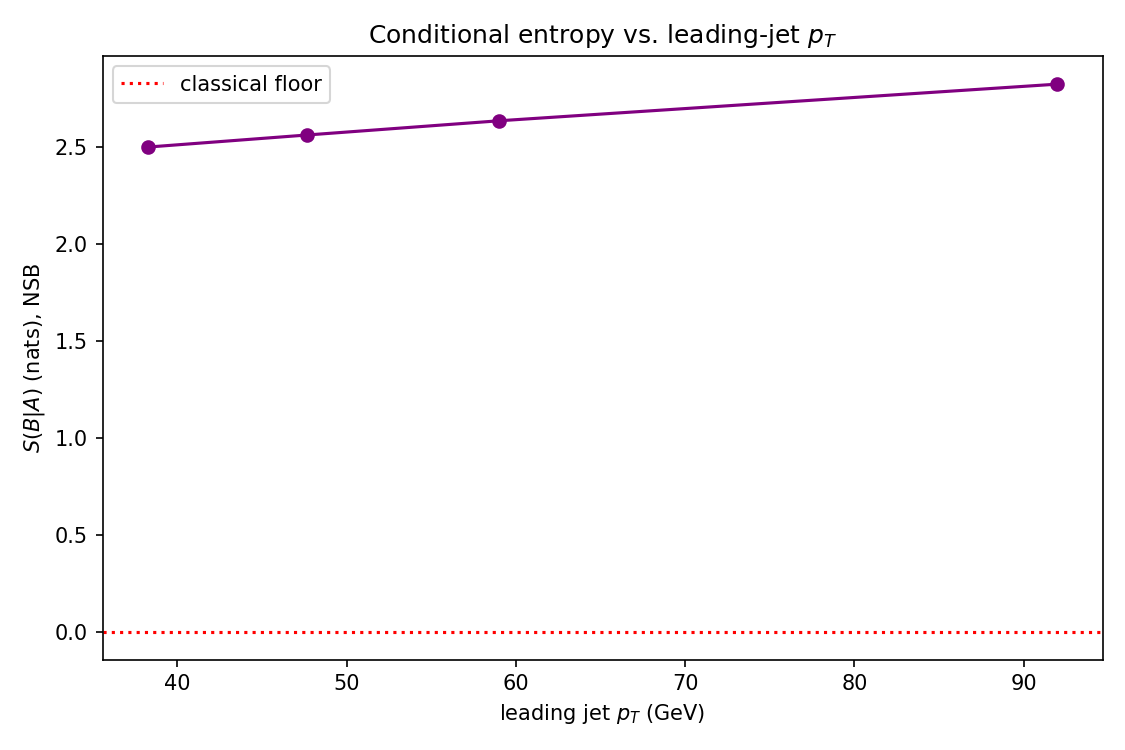
\includegraphics[width=0.8\textwidth]{figs/dijet_entropy_result_truth_SBA_vs_pt.png}
\caption{PYTHIA~8: $\SBA$ (NSB) vs.\ leading-jet $p_T$.}
\label{fig:py-sba-pt}
\end{figure}

\subsection{Multi-method comparison vs.\ $p_T$}

Figure~\ref{fig:py-method-comparison} overlays naive/Miller--Madow/
shuffle/NSB for $I(A{:}B)$, and naive/Miller--Madow/NSB for $\SBA$ (no
shuffle analogue, Sec.~\ref{sec:nsb}), each with bootstrap error bars
computed by the same unified procedure (Sec.~\ref{sec:sensitivity}). The
bias hierarchy naive~$>$~Miller--Madow~$\gtrsim$~NSB~$\approx$~shuffle
seen on the full sample (Fig.~\ref{fig:py-summary}) persists across
$p_T$ bins, most visibly in the highest-$p_T$ (lowest-statistics) bin,
where naive's upward bias is largest -- exactly the pattern the toy study
predicts for a bin with fewer events and a wider effective alphabet.

\begin{figure}[htb]
\centering
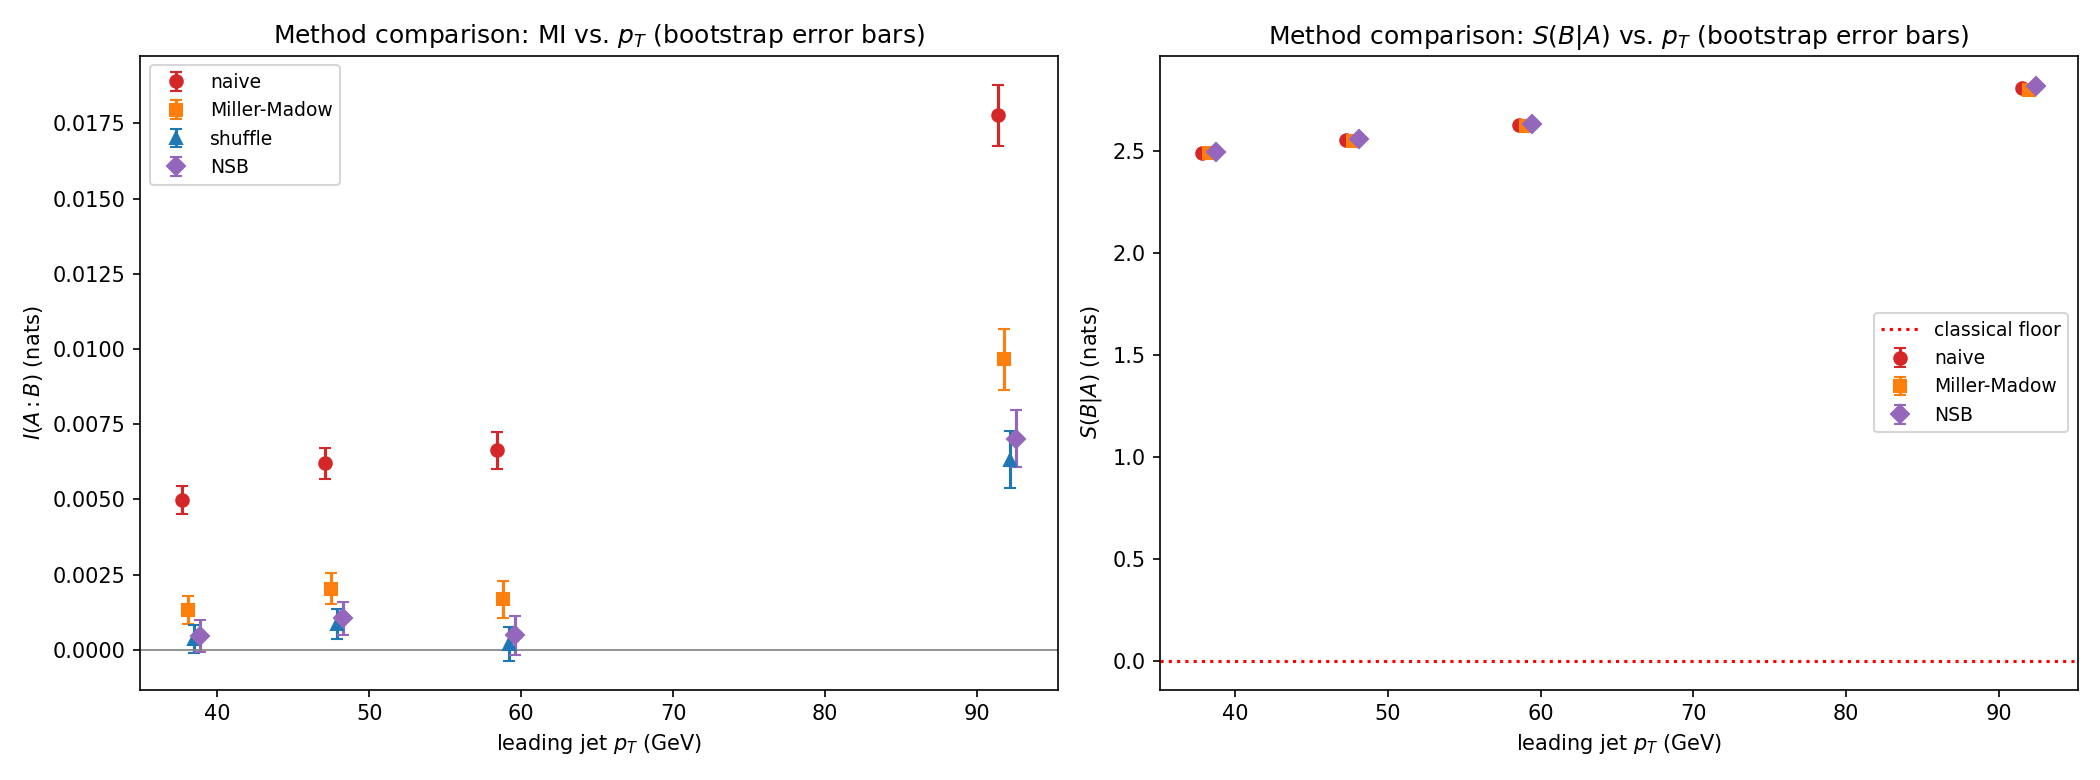
\includegraphics[width=\textwidth]{figs/dijet_entropy_result_truth_method_comparison_vs_pt.png}
\caption{PYTHIA~8: method comparison for $I(A{:}B)$ (left) and $\SBA$
(right) vs.\ leading-jet $p_T$, bootstrap error bars throughout.}
\label{fig:py-method-comparison}
\end{figure}

% =============================================================================
\section{Overall conclusions and next steps}
\label{sec:conclusions}
% =============================================================================

The toy Monte Carlo study (Secs.~\ref{sec:toymc}--\ref{sec:sensitivity})
establishes the estimator methodology and its failure modes under
controlled, known conditions. Section~\ref{sec:pythia} shows the same
pipeline, unmodified, correctly recovers physically-expected behavior
(NBD-like overdispersion, MLLA-consistent multiplicity growth with $p_T$,
the same finite-sample bias shape) on realistic QCD Monte-Carlo output
where no such structure was hand-built in -- a meaningful, if indirect,
validation that the pipeline is measuring real structure rather than an
artifact of the toy model's specific construction.

What this note does \emph{not} yet provide is a validation against a
dataset with an independently \emph{known} $I_{\rm true}$ that is also
calibrated to resemble real jet data (Sec.~\ref{sec:pythia}'s PYTHIA~8
sample has no known truth of its own). A closure test addressing this gap
-- fitting the toy model's Gamma-Poisson structure to real PYTHIA~8
marginals and correlation strength, generating a very large reference
sample from that fitted model to obtain a calibrated pseudo-truth, and
checking recovery (bias and pull-distribution calibration) of all four
estimators at the real dataset's actual statistics -- is in progress at
the time of writing and will be reported separately.

Remaining steps toward the actual STAR measurement: (i) repeat
Sec.~\ref{sec:pythia} at $\sqrt{s}=200$~GeV with STAR-appropriate jet
kinematics rather than the wide-dynamic-range $14$~TeV validation
kinematics used here; (ii) apply the detector-level acceptance and
tracking-efficiency model (already implemented in the generator, not yet
exercised in this note) and repeat the full analysis chain; (iii) once
(i)--(ii) are validated, apply the identical pipeline to real STAR data,
with the sensitivity/detection-threshold machinery of
Sec.~\ref{sec:sensitivity} used to state explicitly, before unblinding,
how large a genuine quantum-correlation excess would need to be to
constitute a significant detection at the actual achieved statistics.

\end{document}

